\chapter{Обзор}
\label{cha:owerview}
Обзоры по численному анализу ГРП можно найти в \cite{GuptaDiss2016, WeberDiss2016, Lecampion2018}. В \cite{Kolawole2020} рассматривается пересечение трещины гидроразрыва с естественными трещинами. Обзор XFEM есть в \cite{PereiraDiss2010,Belytschko2009,Fries2010,Karihaloo2011,Fries2014,flemisch2016,Ahmadkanth2019}.

Литература по моделированию ГРП с применением XFEM в трёхмерной постановке: 
\cite{Gupta2014,Zielonka2014,Gupta2015,GuptaDiss2016,Liu2016,Weber2016,Haddad2016,Gupta2017,Liu2017,Luo2018,Paul2018,Duarte2019,Duarte2020_validation,Duarte2020,Roth2020_1,Roth2020_2,Shi2021}.
\section{Гидравлический разрыв пласта}
Гидравлический разрыв пласта (ГРП) \cite{Magadova2012} -- это физико-гидродинамический процесс, при котором горная порода разрывается по плоскостям минимальной прочности за счет воздействия на пласт давлением, создаваемым закачкой в скважину специальной жидкости разрыва. В образованные трещины с помощью жидкостей разрыва транспортируется расклинивающий материал -- проппант, который, после снятия избыточного давления, закрепляет трещины в раскрытом состоянии. После разрыва давление флюида увеличивает размеры трещины, обеспечивая ее связь с системой естественных природных трещин, не вскрытых скважиной, а также с зонами повышенной проницаемости, расширяя таким образом площадь дренажа скважины и способствуя значительному увеличению ее дебита или приемистости на объектах нагнетания с повышением конечной нефтеотдачи продуктивных пластов.

Цели и области применения ГРП:
\renewcommand{\labelitemi}{$\bullet$}
\begin{itemize}
\item
интенсификация добычи из скважин, в первую очередь с интенсивно кольматированной призабойной зоной, увеличение эффективного радиуса за счет создания высокопроводящих трещин ограниченной длины в средне- и высокопроницаемых пластах, а также в низкопроницаемых достаточно однородных коллекторах;
\item
обеспечение гидродинамической связи скважины с системой естественных трещин пласта и расширение зоны дренирования;
\item
ввод в разработку низкопроницаемых залежей с потенциальным дебитом скважин в 2-3 раза ниже уровня рентабельной добычи и перевод забалансовых запасов в промышленные;
\item
разработка сложных расчлененных и неоднородных пластов, характеризующихся высокой степенью прерывистости, на основе комплексной оптимизации системы разработки с целью обеспечения гидродинамического взаимодействия пласта и системы скважин с трещинами гидраразрыва для увеличения темпа отбора извлекаемых запасов, повышения нефтеотдачи за счет вовлечения в активную разработку слабодренируемых зон и прослоев и увеличения охвата пласта воздействием.
\end{itemize}

Кислотный ГРП предполагает последовательный разрыв пласта полисахарядным гелем и закачку кислотного состава. В качестве жидкости для гидраразрыва могут использоваться прямые и обратные кислотосодержащие эмульсии или полимерные кислотные гели на водной основе.

При обычном ГРП скорость нагружения пород не превышает $1$ МПа/с, а в результате локального взрыва (импульсный ГРП) достигает $10^7$ МПа/с с чередующейся серией затухающих гидраударов скважинной жидкости. В настоящее время существует ряд методов создания щадящих пролонгированных взрывов в скважине с импульсами давления $10^1-10^7$ МПа/с. Как правило, импульсный разрыв формирует сеть горизонтальных коротких трещин. Кроме того, последующее
проведение ГРП с закреплением проппантом существенно снижает давление разрыва горных пород и формирует более раскрытые и протяженные трещины.

Согласно промысловой практике, при глубине залегания продуктивного пласта до 200м в процессе ГРП формируются горизонтальные трещины, а на глубине более 400м -- вертикальные. На промежуточных глубинах ориентация трещин определяется анизотропией пород. Образование горизонтальных трещин предполагается в вертикальных скважинах с протяженной толщиной однородных по прочности пород и ограниченным интервалом перфорации. Радиальную конфигурацию приобретают вертикальные трещины в горизонтальных скважинах (многостадийный ГРП).

Кроме того, природные трещины по многочисленным анализам промысловых результатов бурения и освоения скважин в подавляющем количестве имеют вертикальную ориентацию.

Этапы ГРП:
\begin{itemize}
\item
закачка жидкости разрыва для образования трещин;
\item
закачка жидкости с проппантом;
\item
закачка жидкости для продавливания проппанта в трещины.
\end{itemize}

\begin{figure}[h!]
	%\centering
	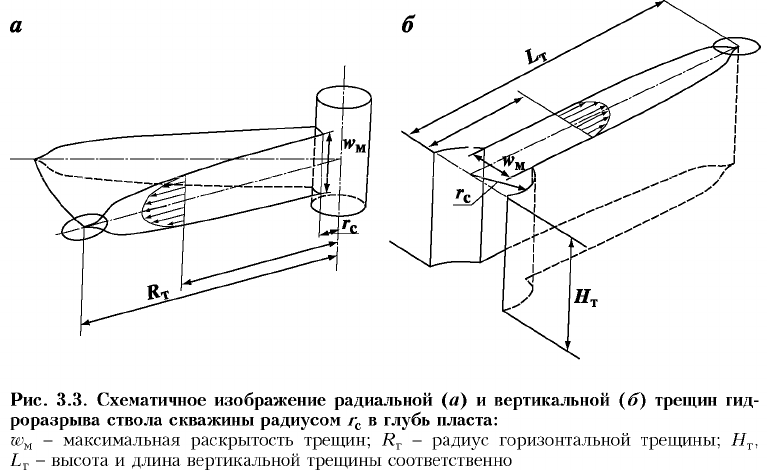
\includegraphics[height=0.4\textheight]{pictures/crack_g_v.png}
	\caption{ [1].
	}
	\label{fig:introduction1}
\end{figure}

\newpage
\section{Упругость}
\subsection{Уравнения равновесия}
В статьях \cite{Gupta2014,Gupta2015,Gupta2017,Duarte2019,Duarte2020_validation} используются уравнения равновесия
\begin{equation}
\int_{\Omega} \sigma:\varepsilon\,d\Omega=
\int_{\partial\Omega} \bar{t}\cdot v\,d\Gamma+
\int_{\Gamma_c^+} \bar{t}_c^+ \cdot \left(v^+-v^-\right)\,d\Gamma,
\label{F:F_XFEM_Governing}
\end{equation}
где $v$ -- пробная функция, $\bar{t}$ -- давление на границе тела $\Omega$, $v^+-v^-$ -- скачок перемещения через границу трещины, $\bar{t}_c^+=-\bar{t}_c^-$ -- давление на поверхность трещины.
\subsection{Базисные функциии}
В XFEM стандартный базис Лагранжа расширяется разрывными функциями:
\begin{equation}
\Delta \mathbf{u}^h\left(\mathbf{x}\right)=
\sum_{n\in N_{nodes}}\sum_{m\in M_{n}}\psi_{nm} \mathbf{a}_{nm},
%\sum_{n=1}^{N}\mathbf{q}_{nm}\varphi_{n}\left(\mathbf{x}\right)
%+\sum_{n=1}^{N}a_{(3n+k-3)}\varphi_{n}\left(\mathbf{x}\right)\left(H\left(\mathbf{x}\right)-H\left(\mathbf{x}_n\right)\right),
\label{F:F_XFEM_appr}
\end{equation}
\begin{equation}
\psi_{nm}=\varphi_n\left(\mathbf{x}\right)\psi_m\left(\mathbf{x}\right)
\label{F:F_XFEM_appr2}
\end{equation}
где $\varphi_{n}$ -- лагранжевы функции формы, $\psi_m\left(\mathbf{x}\right) = 1$ для базисных функций Лагранжа, $\psi_m\left(\mathbf{x}\right)=\psi_m^{enr}\left(\mathbf{x}\right)-\psi_m^{enr}\left(\mathbf{x}_n\right)$ для функций обогащения. $N_{nodes}$ -- множество узлов сетки, $M_{n}$ -- множество степеней свободы узла $n$ (по каждой из координат).

Для задания сильного разрыва вводится функция знака
\begin{equation}
\psi^{enr}=sgn\left(\mathbf{x}\right)=
\begin{cases}
-1 \: \mathrm{if} \: g\left(\mathbf{x}\right)<0\\
+1 \: \mathrm{if} \: g\left(\mathbf{x}\right)>0,\\
\end{cases}
\label{F:F_Hev}
\end{equation}
или Хевисайда
\begin{equation}
\psi^{enr}=H\left(\mathbf{x}\right)=
\begin{cases}
-1 \: \mathrm{if} \: g\left(\mathbf{x}\right)<0\\
0 \: \mathrm{if} \: g\left(\mathbf{x}\right)>0,\\
\end{cases}
\label{F:F_Hev2}
\end{equation}
что приводит к тому же результату. Случай нескольких трещин в одном КЭ рассмотрен в \cite{Moes2013,Moes2016,Moes2017,Paul2018}

Чтобы около фронта трещины в базисе содержалось точное решение линейно-упругой теории разрушения (LEFM), добавляются функции
\begin{equation}
\psi_m^{enr}\left(\mathbf{x}\right)\in\left\lbrace
\sqrt{r}\,\mathrm{sin}\frac{\theta}{2},
\sqrt{r}\,\mathrm{cos}\frac{\theta}{2},
\sqrt{r}\,\mathrm{sin}\frac{\theta}{2}\,\mathrm{sin}\theta,
\sqrt{r}\,\mathrm{cos}\frac{\theta}{2}\,\mathrm{sin}\theta\right\rbrace,
\label{F:F_Williams1}
\end{equation}
где $g\left(\mathbf{x}\right)$ -- функция расстояния от точки $\mathbf{x}$ до поверхности трещины (положительная с одной стороны трещины и отрицательная с другой стороны трещины); $r\left(\mathbf{x}\right)=\left| g\left(\mathbf{x}\right)\right|$; $\theta\left(\mathbf{x}\right)$ -- угол, под которым видна плоскость трещины из точки $\mathbf{x}$.

Функции \eqref{F:F_Williams1} получаются из асимптотического решения Вильямса \cite{Williams1961} и применялись в \cite{Belytschko1999} для XFEM. Эквивалентные альтернативы обогащений обсуждаются в \cite{Gupta2013,Gupta2015_sgfem}.

Функции обогащения для ортотропного материала: \cite{Asadpoure2007,Hattori2012}.

В смешанном подходе для упругопластического анализа трещин \cite{Feulvarch2020} вводится дополнительное поле давления и аппроксимирующие его функции около фронта трещины \cite{Westergaard1939}
\begin{equation}
\psi_m^{enr}\left(\mathbf{x}\right)\in\left\lbrace
\frac{1}{\sqrt{r}}\,\mathrm{cos}\frac{\theta}{2},
\frac{1}{\sqrt{r}}\,\mathrm{sin}\frac{\theta}{2},
\right\rbrace,
\label{F:F_Westergaard}
\end{equation}

\subsection{Интегрирование}
Разрывную функцию можно проинтегрировать по КЭ, разделив его на подобласти, на которых функция непрерывна, тогда можно будет применить квадратурные формулы Гаусса на каждой подобласти \cite{Fries2010,GuptaDiss2016,Weber2016}. Шестигранник можно разрезать на 5 тетраэдров (не единственным способом). Чтобы сгустить точки Гаусса к фронту трещины, тетраэдр можно интегрировать как шестигранник, используя отображение \cite{Minnebo2012}, или разбивать поверхность пересечения трещины с тетраэдром на тетраэдры \cite{GuptaDiss2016}. Разбиение шестигранника на призмы для случая вертикальной трещины с классификацией случаев рассмотрено в \cite{Nagashima2020}.

Другой подход, пригодный для интегрирования функций Хевисайда, основан на усреднении объёма и квадратурных формулах Гаусса \cite{Belytschko1988,Nikolakopoulos2020}.

\section{Рост трещины (LEFM)}
\subsection{Направление роста трещины}
Направление роста трещины можно задать при помощи угла в координатах фронта трещины: углом изгиба $\theta_0$ и углом закручивания $\varphi_0$ при помощи критерия максимума тангенциального напряжения Schollmann \cite{Schollmann2002}:
\begin{equation}
\left.\frac{\partial\sigma_1}{\partial\theta}=0\right|_{\theta=\theta_0},\,\left.\frac{\partial^2\sigma_1}{\partial\theta^2}<0\right|_{\theta=\theta_0},
\label{F:F_Schollmann1}
\end{equation}
\begin{equation}
\varphi_0=\frac{1}{2}\mathrm{arctan}\left( \frac{2\tau_{\theta z}\left(\theta_0 \right)}{\sigma_\theta\left(\theta_0 \right)-\sigma_z\left(\theta_0 \right)} \right),
\label{F:F_Schollmann2}
\end{equation}
где $\sigma_1$ -- максимальное главное напряжение; $\sigma_\theta$, $\tau_{\theta z}$ и $\sigma_\theta$ -- компоненты тензора напряжений в цилиндрической системе координат, заданной относительно фронта трещины.

Процедура вычисления эффективного направления $\theta^*$ с учётом углов $\theta_0$ и $\varphi_0$ дана в \cite{PereiraDiss2010}.
\subsection{Величина продвижения фронта при росте трещины}
В случае хрупкого разрушения, величину продвижения фронта (для некоторого узла) можно задать критерием Irwin \cite{Irwin1997} в регуляризованном виде, предложенном \cite{Lazarus2003}, который использовался в \cite{Gupta2017,Duarte2019,Duarte2020_validation,Duarte2020}:
\begin{equation}
\Delta a =
\begin{cases}
0, & \mathrm{}\;0\leqslant \frac{K_{I,eq}}{K_{Ic}} < 1-\alpha-\beta \\
\frac{\Delta a_{max}}{\beta}\left(  \frac{K_{I,eq}}{K_{Ic}} - \left( 1-\alpha-\beta \right) \right) , & \mathrm{}\;1-\alpha-\beta \leqslant \frac{K_{I,eq}}{K_{Ic}} < 1-\alpha \\
\Delta a_{max}, & \mathrm{}\;1-\alpha \leqslant \frac{K_{I,eq}}{K_{Ic}} \leqslant 1+\alpha \\
\end{cases}
\label{F:F_propogation1}
\end{equation}
где
\begin{equation}
\begin{gathered}
K_{I,eq} = \frac{1}{2}\mathrm{cos}\left( \frac{\theta_0}{2} \right)
\left(K_I\,\mathrm{cos}^2 \left(\frac{\theta_0}{2}\right)-\frac{3}{2}K_{II}\,\mathrm{sin} \left(\theta_0\right) \right. \\ 
\left. +\sqrt{\left(K_I\,\mathrm{cos}^2 \left(\frac{\theta_0}{2}\right)-\frac{3}{2}K_{II}\,\mathrm{sin} \left(\theta_0\right)\right)^2+4K_{III}^2}
\right),
\end{gathered}
\label{F:F_propogation2}
\end{equation}
$K_{I},\,K_{II},\,K_{III}$ -- коэффициенты интенсивностей напряжений (КИН, открывающая (I), поперечно-сдвиговая (II) и продольно-сдвиговая (III) моды деформаций), $K_{I,eq}$ -- эквивалентная мода I, $K_{Ic}$ -- трещиностойкость. $\alpha,\,\beta,\,\Delta a_{max}$ -- параметры материала.

В \cite{Gupta2014} применялись критерии
\begin{equation}
\Delta a =
\begin{cases}
0, & \mathrm{}\; K_{I,eq}\leqslant K_{Ic} \\
\Delta a_{max}\left(\frac{K_{I,eq}-K_{Ic}}{K_{I,eq}^{max}-K_{Ic}}\right)^m, & \mathrm{}\; K_{I,eq}>K_{Ic}\\
\end{cases}
\label{F:F_propogation3}
\end{equation}
и
\begin{equation}
\Delta a = \Delta a_{max}\left(\frac{K_{I,eq}}{K_{I,eq}^{max}}\right)^m
\label{F:F_propogation4}
\end{equation}
где $\Delta a_{max}$ и $m$ -- параметры материала.
\subsection{Вычисление SIF}
Сравнение методов вычисления КИН \cite{Gupta2017_SIF} показывает, что предпочтительным является Displacement Correlation Method (DCM), который основан на связи перемещений и КИН:
\begin{equation}
\begin{gathered}
K_{I,r}=\sqrt{\frac{2\pi}{r}}\left(\frac{\mu}{\kappa+1}\right)\Delta v\left(r\right), \\
K_{II,r}=\sqrt{\frac{2\pi}{r}}\left(\frac{\mu}{\kappa+1}\right)\Delta u\left(r\right), \\
K_{III,r}=\sqrt{\frac{2\pi}{r}}\left(\frac{\mu}{4}\right)\Delta w\left(r\right), \\
\end{gathered}
\label{F:DCM1}
\end{equation}
где $\kappa=3-4\nu$. $\Delta u,\,\Delta v,\,\Delta w$ -- компоненты скачка вектора перемещений ($\theta=\pm\pi$) в системе координат, связанной с фронтом трещины.
\begin{figure}[h!]
	\centering
	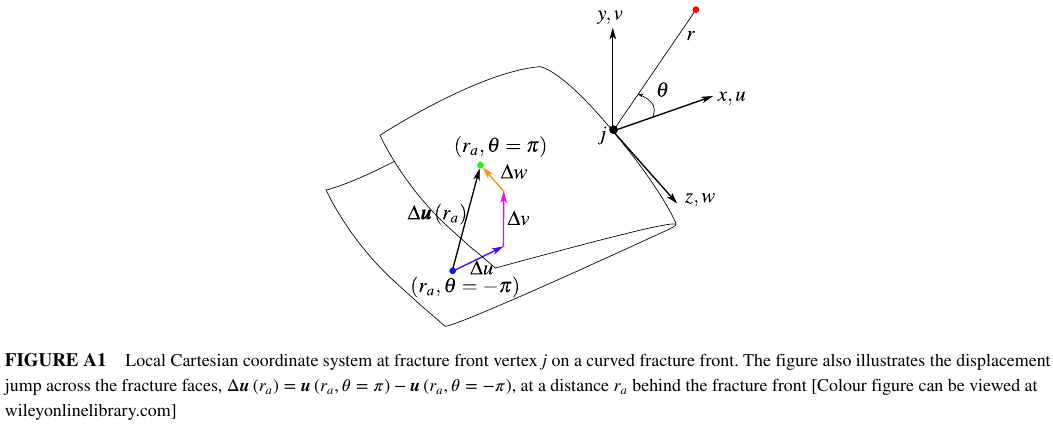
\includegraphics[height=0.2\textheight]{pictures/SIF.png}
	\caption{из \cite{Gupta2017}}
	\label{fig:SIF}
\end{figure}

Путём экстраполяции \cite{Dirgantara2002} можно получить КИН в вершине трещины:
\begin{equation}
\begin{gathered}
K_{I}=\frac{r_b}{r_b-r_a}\left(K_{I,r_a}-\frac{r_a}{r_b}K_{I,r_b}\right), \\
K_{II}=\frac{r_b}{r_b-r_a}\left(K_{II,r_a}-\frac{r_a}{r_b}K_{II,r_b}\right), \\
K_{III}=\frac{r_b}{r_b-r_a}\left(K_{III,r_a}-\frac{r_a}{r_b}K_{III,r_b}\right), \\
\end{gathered}
\label{F:DCM2}
\end{equation}
Этот метод наиболее просто реализовать. Требуется дробление сетки вблизи фронта трещины для обеспечения хорошей точности.
\section{Рост трещины (CZM)}
Модель сил сцепления (cohesive zone model) применялась в статьях \cite{Liu2016, Liu2017, Paul2018}, а также с использованием ABAQUS в статьях \cite{Zielonka2014, Haddad2016}.

Направление роста трещины задаётся формулами \eqref{F:F_Schollmann1}, \eqref{F:F_Schollmann2}.

Рост трещины в модели сил сцепления определяется силами сцепления $t_c$, действующими на поверхности трещины
\begin{equation}
t_c =
\begin{cases}
T_{ts}\frac{w}{g_0}, & \mathrm{}\; w\leqslant g_0 \\
T_{ts}\frac{g_1-w}{g_1-g_0} , & \mathrm{}\; g_0<w\leqslant g_1\\
0, & \mathrm{}\; w>g_1 \\
\end{cases}
\label{F:CZM}
\end{equation}
\begin{figure}[h!]
	\centering
	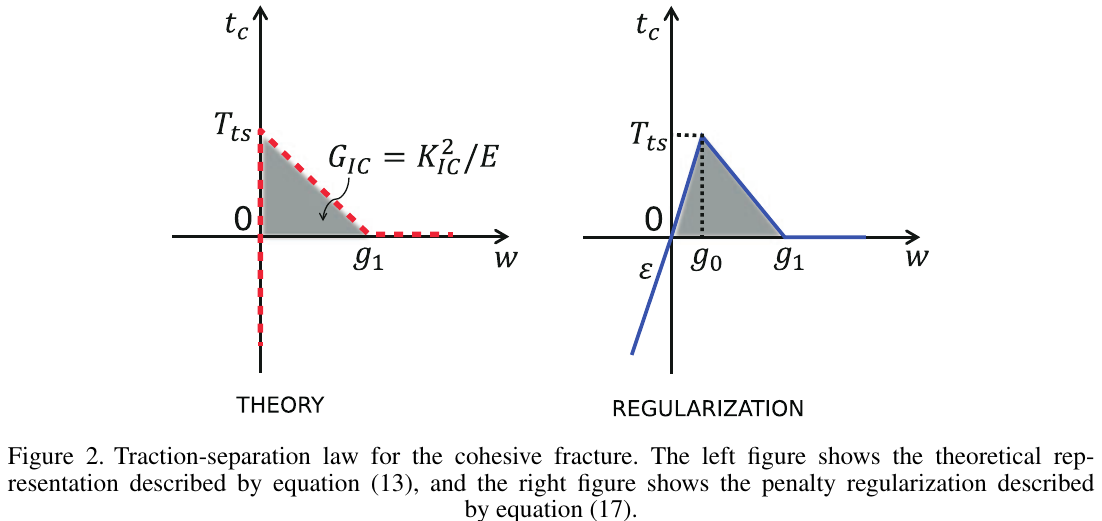
\includegraphics[height=0.3\textheight]{pictures/CZM_ts.png}
	\caption{из \cite{Liu2016}}
	\label{fig:CZM_ts}
\end{figure}
Связь параметра $g_2$ с вязкостью разрушения $K_{IC}$ определяется формулой \cite{Irwin1997}
\begin{equation}
K_{IC}=\sqrt{G_{IC}\frac{E}{1-\nu^2}}
\label{F:CZM1}
\end{equation}
где $G_{IC}$ -- энергии хрупкого разрушения:
\begin{equation}
G_{IC}=\frac{1}{2}T_{ts}g_1
\label{F:CZM2}
\end{equation}
Величина упругого участка $g_0$ считается малой:
\begin{equation}
g_0=\frac{T_{ts}}{\epsilon},\;\epsilon\gg E
\label{F:CZM3}
\end{equation}
Контакт между сторонами трещины автоматически учитывается дополнительным участком кривой при $w<0$.

В статьях \cite{Roth2020_1, Roth2020_2} в форме сил сцепления записана continuous damage model.

\section{Контакт, разветвление трещин, учёт природных трещин}
Для учёта контакта применимы стандартные методы типа штрафа \cite{GuptaDiss2016}.
Задание разветвлённых трещин (“junction” функции), взаимодействие между трещинами \cite{Moes2013,Moes2016,Moes2017,Paul2018}.
\section{Гидромеханика}
В статьях \cite{Gupta2015,Gupta2017,Duarte2019,Duarte2020} жидкость внутри трещины считается ньютоновской и несжимаемой, без учета инерционных и гравитационных эффектов, тогда закон сохранения массы приводит к уравнению
\begin{equation}
\int_{\Gamma_c}\left(\frac{\partial w}{\partial t}+q_L-q_I\right)v\,d\Gamma_c
-\int_{\Gamma_c}\mathbf{q}\cdot\nabla_{\overline{\mathbf{x}}}v\,d\Gamma_c
+\int_{\partial\Gamma_c^N}v\overline{q}\,ds=0
\label{F:F_flow1}
\end{equation}
где $w=\left(\mathbf{u}^+-\mathbf{u}^-\right)\cdot \mathbf{n}^-$ -- ширина трещины, $q_L$ -- утечка через границы трещины, $q_I$ -- скорость закачки жидкости, $v$ -- пробная функция, $\overline{q}$ -- поток по нормали к границе трещины $\partial\Gamma_c^N$, $\mathbf{q}$ -- поток внутри трещины, заданный кубическим законом Пуазейля
\begin{equation}
\mathbf{q} = -\frac{w^3}{12\mu}\nabla_{\overline{\mathbf{x}}}p,
\label{F:F_flow2}
\end{equation}
где $\mu$ -- вязкость жидкости,
\begin{equation}
\nabla_{\overline{\mathbf{x}}}=
 \frac{\partial}{\partial\overline{x}_1}\,\overline{\mathbf{e}}_1
+\frac{\partial}{\partial\overline{x}_2}\,\overline{\mathbf{e}}_2
\label{F:F_flow3}
\end{equation}
Каждая система координат с базовыми векторами $\left\lbrace \overline{\mathbf{e}}_1,\;\overline{\mathbf{e}}_2\right\rbrace $ и вектором положения $\left( \overline{x}_1,\;\overline{x}_2\right) $ связана с конечным элементом сетки, используемой для решения уравнения \eqref{F:F_flow1}.

\section{*Связанная гидро-механическая задача}
Gupta2017
?Дискретизация по времени
Пороупругость, leak-off Carter model (жидкость уходит в породу)
fluid lag (задержка жидкости из-за пористого включения в трещине)

Cohesive zone method (CZM), traction-separation constitutive law \cite{Moes2016}
viscosity- (M ) ... toughness- dominated (K) regime, GFEM enr.



\section{Сравнительный обзор статей}
\begin{landscape}
\begin{table}[h!]
	\caption{Обзор литературы}
	%\ctable [doinside=\small]
	%\begin{tabular}{|p{5.3cm}|c|p{7cm}|}
	%	\hline
	%	Параметр      & Обозначение & Значение  \\
	%	\hline
	%\begin{tabular}{|p{5.3cm}|c|p{7cm}|}
	%\small
	\footnotesize
	\begin{tabular}{|l|c|c|c|c|c|c|c|c|c|}
		\hline
		Источник & Год & Упругость & Обогащение & Рост трещины & Жидкость & Связанность & Разветвление & Контакт & Ком. CAE? \\
		\hline
		GD\cite{Gupta2014}&2014&упругость \eqref{F:F_XFEM_Governing}&Хевисайда, в вершине&Irwin \eqref{F:F_propogation3}, \eqref{F:F_propogation4} &$p=const$&---&---&---&---\\
		\hline
		GD\cite{Gupta2015}&2015&---//---&---//---&статика&\eqref{F:F_flow1}&м. Ньютона-Рафсона&---&---&---\\
		\hline
		GD\cite{Gupta2017}&2017&---//---&---//---&Irwin \eqref{F:F_propogation1}&\eqref{F:F_flow1}&м. Ньютона-Рафсона&---&---&---\\
		\hline
		GD\cite{Duarte2019}&2019&---//---&---//---&Irwin \eqref{F:F_propogation1}&\eqref{F:F_flow1}&м. Ньютона-Рафсона&---&---&---\\
		\hline
		GD\cite{Duarte2020_validation}&2020&---//---&---//---&Irwin \eqref{F:F_propogation3}&---&---&---&---&---\\
		\hline
		GD\cite{Duarte2020}&2020&---//---&---//---&Irwin \eqref{F:F_propogation1}&\eqref{F:F_flow1}&м. Ньютона-Рафсона&---&---&---\\
		\hline
		
		%CZM
		Liu\cite{Liu2016}&2016&упругость \eqref{F:F_XFEM_Governing}&Хевисайда&CZM \eqref{F:CZM}&\eqref{F:F_flow1}&м. Ньютона-Рафсона&---&включён в CZM&---\\
		\hline
		Liu\cite{Liu2017}&2017&упругость \eqref{F:F_XFEM_Governing}&Хевисайда&CZM \eqref{F:CZM}&\eqref{F:F_flow1}&м. Ньютона-Рафсона&---&включён в CZM&---\\
		\hline		
		\cite{Paul2018}&2018&пороупругость&Хевисайда, junction&CZM без рег.&\eqref{F:F_flow1}&расш. м. Лагранжа&разветвление&&---\\
		\hline
		
		
		\cite{Luo2018}&2018&&&&&&&&---\\
		\hline
%		Diss\cite{WeberDiss2016}&2016&&&&&&&&---\\
%		\hline

		Roth\cite{Roth2020_1}&2020&пороупругость&Хевисайда&CDM ч/з $t_c$&...&м. Ньютона-Рафсона&---&м. штрафа&---\\
		\hline
		Roth\cite{Roth2020_2}&2020&пороупругость&Хевисайда&CDM ч/з $t_c$&...&м. Ньютона-Рафсона&---&м. штрафа&---\\
		\hline

		%CZM ABAQUS 
		\cite{Zielonka2014}&2014&пороупругость&Хевисайда, ф. узлы&CZM \eqref{F:CZM}&\eqref{F:F_flow1}&&---&---&ABAQUS\\
		\hline
		\cite{Haddad2016}&2016&пороупругость&Хевисайда, ф. узлы&CZM \eqref{F:CZM}&&&пересечение&---&ABAQUS\\
		\hline
		

		
		
		\hline
	\end{tabular}
	\label{tab:lit_owerview}
\end{table}

\end{landscape}


%\newpage




%Неплоское распространение трещин в трехмерном пространстве, смоделированное с помощью XFEM, было представлено в %[Gupta2014]




%%% Local Variables:
%%% mode: latex
%%% TeX-master: "rpz"
%%% End:
